\documentclass[11pt]{article}
\usepackage[letterpaper,top=.93in,bottom=.92in,left=1.03in,right=1.03in]{geometry}
\usepackage{amsmath,amssymb,amsthm,booktabs,array,tabularx,graphicx,xcolor,microtype,fancyhdr,hyperref,titlesec}
\definecolor{inkblue}{HTML}{214D62}
\hypersetup{colorlinks=true,linkcolor=inkblue,urlcolor=inkblue,citecolor=inkblue,pdftitle={Finite observations in constructive arithmetic},pdfauthor={Research report prepared for Vladimir Reshetnikov}}
\titleformat{\section}{\normalfont\Large\bfseries\color{inkblue}}{\thesection}{.65em}{}
\titleformat{\subsection}{\normalfont\large\bfseries}{\thesubsection}{.55em}{}
\titlespacing*{\section}{0pt}{2.0ex plus .6ex minus .2ex}{1.1ex plus .3ex}
\titlespacing*{\subsection}{0pt}{1.8ex plus .5ex minus .2ex}{.7ex plus .2ex}
\pagestyle{fancy}\fancyhf{}\fancyhead[L]{\small Finite observations in constructive arithmetic}
\fancyhead[R]{\small\thepage}\renewcommand{\headrulewidth}{.3pt}
\setlength{\headheight}{14pt}\setlength{\emergencystretch}{1.6em}\raggedbottom
\newtheorem{theorem}{Theorem}[section]\newtheorem{lemma}[theorem]{Lemma}\newtheorem{corollary}[theorem]{Corollary}
\newcommand{\N}{\mathbb N}\newcommand{\Q}{\mathbb Q}\newcommand{\R}{\mathbb R}
\newcommand{\Lip}{\operatorname{Lip}}\newcommand{\ipra}{\mathsf{iPRA}}
\newcommand{\repourl}{https://github.com/VladimirReshetnikov/ProveIt/blob/5f3be02388442f16487d2dc5c2529961dd783d2b/Logic/PrimitiveRecursiveArithmetic}
\newcommand{\repo}[2]{\href{\repourl/#1}{#2}}
\begin{document}
\thispagestyle{empty}
\noindent{\sffamily\small\color{inkblue} MATHEMATICAL LOGIC\quad /\quad CONSTRUCTIVE ANALYSIS}\par
\vspace{.8em}\noindent{\LARGE\bfseries Finite observations in constructive arithmetic}\par
\vspace{.4em}\noindent{\large Function spaces, metric structures, nerves and residues in iPRA}\par
\vspace{.6em}\noindent{\small Research report prepared for Vladimir Reshetnikov\hfill 20 November 2026}\par
\vspace{.8em}\hrule\vspace{.8em}
\noindent How can a first-order arithmetic proof make a statement about \emph{all functions} on a continuum? For bounded scalar functions with a prescribed Lipschitz constant, one can construct a finite net whose members are themselves functions of that class. Their uniform distances are computable exactly from their defining lists of points. The construction can be iterated, so a variable ranging over Lipschitz functionals can also be eliminated to any requested accuracy. We give the coverage proof, the arithmetic interpretation of these quantifiers, and an exact minimax calculation.
\par\smallskip
Three applications show how the interpretation changes with the mathematics. Two-sided correspondences transport a fragment of continuous logic with no growth of error through quantifiers. Finite unions of rational boxes admit explicit nerve equivalences with computable homotopies, including at tangencies. A rational-collar argument transfers a residue theorem to positively isolated singularities whose centres are given by primitive recursive names.
\par\smallskip
The Lean files include a checked derivation constructor in ProveIt's embedded calculus and checked mathematical kernels for the examples. The full arithmetic reification of the applications is specified in the paper and remains to be mechanized.
\vspace{.6em}
\setcounter{tocdepth}{1}\tableofcontents
\clearpage
\section{What an embedding asserts}
\label{sec:base}

The radius of the geodesic circle of circumference two is one. Its expression $\inf_x\sup_y d(x,y)=1$ quantifies over a continuum twice. A finite calculation at one resolution only bounds the value. To express the equality in arithmetic we need a uniform procedure for producing the bounds and a proof of their accuracy at every resolution. Showing that every quantified point can be matched, in the correct direction, is the part that justifies the two quantifiers.

\subsection{Theory, numerical data and proof obligations}

We use the repository's first-order intuitionistic arithmetic with equality, successor axioms, a symbol and defining equations for every specified primitive recursive (PR) definition, and induction on quantifier-free formulas with numerical parameters. Its Lean judgment is $\Gamma\vdash_{\mathsf{PRAAx}}\phi$. The \repo{README.md}{directory guide} distinguishes checked object derivations from the research packets in \texttt{docs/proofs}. A Lean proof about rational numbers can validate an estimate, while an object proof constructs a derivation using this particular induction schema.

Here is a numerical coding sufficient throughout. Use $0$ for the empty list and $2^a(2b+1)$ for a list with head $a$ and tail code $b$. On a positive code $c$, test divisibility by $2^i$ for $i\le c$ to recover its exponent, then divide to recover the tail. Each positive tail step strictly decreases the code, so $c$ iterations suffice. Code signed integers by parity, rationals by a signed numerator and positive denominator, and pairs and matrices by lists with shape checks. Comparison cross-multiplies positive denominators. Malformed codes have default outputs, and theorems include the necessary validity guards. A finite Cartesian power uses a radix representation or iterated list indexing.

A bounded formula in these predicates has a PR bit. For example, for a Boolean $b(i,p)$ define $u(0,p)=1$ and $u(j+1,p)=u(j,p)b(j,p)$. From $u(j,p)=1$ recover each required factor by fixing its index and inducting on the length of the suffix, using $ab=1\Rightarrow a=b=1$ for bits. Conversely, under the universal premise each successive factor is one and induction uses the equation $u(\min(i,j),p)=1$ for the fixed terminal $j$. A bounded existential uses a first-success register, with the bound itself as sentinel. This replaces bounded statements \emph{inside} loop invariants by an equality to $1$. The repository implements the discipline in \repo{Derivations/Lean/IPRADerivations/Foundations/BoundedSyntax.lean}{BoundedSyntax} and \repo{Derivations/Lean/IPRADerivations/Foundations/BoundedReflection.lean}{BoundedReflection}. A hypothesis valid at every precision can remain in the context throughout an induction. Only the invariant needs to be quantifier-free.

\paragraph{Names and equality.}
Let $D$ be a nonempty set of valid numerical codes with a rational PR pseudometric $d$. Require arithmetic proofs of the rational metric axioms on valid codes. A regular name is a fixed PR family $a(p,k)\in D$ satisfying
\[
 d(a(p,k),a(p,l))\le 2^{-k}+2^{-l}.
\]
Numerical parameters $p$ can be quantified in iPRA. A different family of names gives another instance of the theorem scheme. Two names represent the same point if the same inequality holds across both families at all pairs of indices. For transitivity, compare through the middle name at precision $j$ and remove the extra $2^{1-j}$. In detail, if rationals $u>v$, their difference is at least the inverse of the product of their denominators. Choose $j$ by bounded search so the extra slack is smaller. Thus a non-strict rational bound with arbitrary dyadic slack implies the bound itself, intuitionistically.

A scalar $z$ has rational approximations $z_k$. The assertion $z\le q$ means $\forall k\,(z_k\le q+2^{-k})$ and $q<z$ has positive witnesses $q<z_k-2^{-k}$. For $|z-w|\le e$, use $|z_k-w_l|\le e+2^{-k}+2^{-l}$ for every $k,l$. A complex name uses rational taxicab distance. Equality of names is generally an unbounded predicate. Algorithms below branch on rational comparisons.

\paragraph{Presenting a spatial sort.}
A net of radius $2^{-r}$ consists of a nonempty PR list $D_r=(a_{r,i})_{i<N(r)}$ and a coverage proof for each $x\in D$. Bounded search on the exact distances returns an $i<N(r)$ with $d(x,a_{r,i})\le2^{-r}$. For a named point sample it more finely and use a finer net, splitting the error between the two operations. At precision $r+2$ each error is at most $2^{-r-2}$. Thus the dense nets cover the completion after a precision shift even if an exact boundary test on names is unavailable. An evaluator on the dense carrier with Lipschitz bound $L$ extends to names: read the input to error at most $2^{-k-2}/\max(1,L)$ and evaluate to error $2^{-k-2}$. Cross-stage comparison gives a regular output independent of the input name. A PR modulus works in place of $L$. For tuples use the maximum distance.

\paragraph{Scope of quantification.}
An analytic formula in this report denotes its family of rational accuracy statements for specified presentations and operations. An upper bound for all $L$-Lipschitz functions has an arithmetical statement about finite net codes, an instance for each presented admissible function, and an external interpretation on the completed space. We prove the connection. Extending the interpretation to all classical functions requires no number indexing each one. Indeed if $U(e,x)$ were a PR evaluator for every PR program, $x\mapsto U(x,x)+1$ would have an index $e$, giving a contradiction at $x=e$. Our uniform algorithms evaluate fixed grammars of tables and envelopes or fixed procedures on numerical parameters.

\subsection{Eliminating a compact quantifier}

Let $D$ have the preceding nets and let a bounded observable $P$ have a joint PR evaluation algorithm on its numerical codes, with regular outputs and a certified uniform continuity modulus. Write $\mu(k)$ for an input precision ensuring an output change at most $2^{-k}$. For requested accuracy $k$, choose a net fine enough for $2^{-k-2}$ oscillation, evaluate all entries to $2^{-k-2}$, and return their maximum $v_k$. Use the domain precision shift above when a completion point is queried. Define a minimum dually.

\begin{lemma}[Quantitative supremum]\label{lem:sup}
The $v_k$ give a regular name for the supremum. A PR selector gives a net entry with value at least $v_k-2^{-k-2}$. The construction is uniform in parameters for which the nets, evaluator and modulus are uniform.
\end{lemma}
\begin{proof}
On the dense carrier every value is at most $v_k+2\cdot2^{-k-2}$: move to a net entry and account for its sample error. At a maximizing entry its actual value is at least $v_k-2^{-k-2}$. Applying the first estimate at the maximizing entry for $l$ gives $v_l\le v_k+2\cdot2^{-k-2}+2^{-l-2}$. Interchanging $k,l$ proves regularity. The limit bounds every value by the first estimate at every precision. Any upper bound dominates the value at each maximizing entry, hence dominates the limit. The numerical versions use arbitrary finite sample margins and the rational-gap argument above. A scan tracks the current maximum and its first attaining index. Its invariant is the conjunction of membership in the prefix, the value equation, and the bounded bit for domination of every prefix entry. Start at the first element. This accounts for the numerical induction. Continuity extends the upper bound to completed points.
\end{proof}

A strict threshold with a supplied margin has a witness at a computable precision. A sequence of maximizing indices can fail to be Cauchy. Section~\ref{sec:var} constructs an exact optimizer in a case where more can be proved.

Products use the maximum distance and the Cartesian product of the two nets. Coverage selects one index per coordinate. Lemma~\ref{lem:sup} now applies down any fixed expression of extrema and uniformly continuous connectives. A modulus in a free parameter passes unchanged through an extremum if the body has it uniformly over the bound variable: take the inequality for each element and compare upper bounds in both directions. Section~\ref{sec:metric-logic} gives a sharper joint estimate from a two-sided correspondence.

\paragraph{A checked logical rule.}
At fixed precision an upper threshold for a maximum has the form $\forall i\,(i<N\to P(i))$ and a lower threshold has the form $\exists i\,(i<N\wedge P(i))$. For a minimum the roles reverse. Suppose target challenges can be carried back by an object term $s$ and source witnesses carried forward by a term $t$. From a derivation of $P(s(y))\to Q(y)$ under a fresh $y$, universal introduction and elimination derive $(\forall x\,P(x))\to\forall y\,Q(y)$. From $P(x)\to Q(t(x))$, eliminate the source existential, introduce $t(x)$, and discharge the opened variable. Iterating these rules through a prefix reduces transport to an arithmetic derivation at a leaf. \texttt{ObjectTransport.lean} implements capture-avoiding substitution under the binders and returns a literal derivation in \texttt{Prf PRAAx}. The application must derive validity of its selected responses and its error bound. Bounds can be included in $P,Q$; interspersed guards use the usual implication and conjunction rules. On nonempty stages an out-of-range challenge can also be mapped to a default valid vertex.

\section{Building nets for spaces of functions}
\label{sec:lipsort}

The repository's \repo{docs/proofs/foundations/ipra_finite_use_framework_2026-11-15/sections/09_compactness.tex}{finite-net transfer theorem} starts with a supplied net. We construct such a net for a function space and compute the pseudometric on its codes. This produces the input for a second application of the same construction to functionals.

Fix a nonempty rational pseudometric presentation $(D,d)$ as in Section~\ref{sec:base}, with its dyadic nets. Write $X$ for the completion and fix a nonnegative rational $L$. The target sort is the space $\Lip_L(X,[0,1])$ of functions satisfying $|f(x)-f(y)|\le Ld(x,y)$, with the uniform distance. A finite code $A$ is a list of pairs $(a,b)$ with $a\in D$ and $b\in\Q\cap[0,1]$. Its value at a rational-carrier point is
\begin{equation}
 G_A(x)=\min\bigl(\{1\}\cup\{b+Ld(x,a):(a,b)\in A\}\bigr).
 \label{eq:cone}
\end{equation}
The empty list represents the constant one. This uses the upper extension formula of McShane for Lipschitz data. We allow mutually inconsistent sample heights and do not require $G_A(a)=b$. This detail makes the enumeration and exact distance calculation work together.\footnote{E. J. McShane, \emph{Extension of range of functions}, Bull. Amer. Math. Soc. 40 (1934), 837--842. \href{https://doi.org/10.1090/S0002-9904-1934-05978-0}{Original article}.}

\begin{lemma}[Distance witnessed by the anchors]\label{lem:anchors}
Every $G_A$ is $[0,1]$-valued and $L$-Lipschitz. Set
\[
 E(A,h)=\max\bigl(\{0\}\cup\{h(a)-b:(a,b)\in A\}\bigr).
\]
For any $[0,1]$-valued $L$-Lipschitz $h$, and $e\ge0$,
\[
  E(A,h)\le e\quad\Longleftrightarrow\quad
      h(x)-G_A(x)\le e\quad\text{for every }x.
\]
In particular, the number
\begin{equation}
 \Delta(A,B)=\max\{E(A,G_B),E(B,G_A)\}                 \label{eq:metric}
\end{equation}
is the exact uniform distance of two finite codes.
\end{lemma}
\begin{proof}
Triangle inequalities show each cone $b+Ld(x,a)$ changes by at most $Ld(x,y)$. A finite minimum of such functions obeys the same bound: every entry at $x$ is at least the corresponding entry at $y$ minus $Ld(x,y)$, and conversely. The constant entry $1$ caps the range, and the heights and distances are nonnegative.

If $E(A,h)\le e$, then for each anchor $h(x)\le h(a)+Ld(x,a)\le b+Ld(x,a)+e$. Also $h(x)\le 1+e$. Minimize the right sides. In the converse direction use $x=a$ and $G_A(a)\le b$. Applying both directions with $h=G_B$ and then $h=G_A$ proves that $\Delta$ bounds all discrepancies and is below every nonnegative such bound. If $\Delta>0$, a maximizing term in one of the lists supplies an actual point of attainment. If $\Delta=0$, all values agree. Symmetry and reflexivity follow directly; apply the pointwise triangle inequality and the bound characterization to get the triangle law for $\Delta$. All operations in \eqref{eq:metric} are rational, including when two different codes have distance zero.
\end{proof}

\begin{theorem}[A primitive recursive inner net]\label{thm:inner}
Let $D_r$ have $N(r)$ entries and radius $\eta=2^{-r}$. For a requested $k$, put
\[
 h=2^{-k-2},\qquad
 r=k+3+\min\{c:2^c\ge\max(1,L)\}.
\]
On the list $D_r$ take all height vectors with entries in $\{0,h,2h,\ldots,1\}$. The resulting $(2^{k+2}+1)^{N(r)}$ codes are members of the Lipschitz ball and cover it in uniform distance with radius at most $2^{-k-1}$. A bounded procedure selects a covering code from the values of its input function at the listed points, each read to absolute error $h/2$.
\end{theorem}
\begin{proof}
Given $f$, round its rational sample at $a$ to the nearest multiple of $h$, resolving exact rational ties towards the lower grid index; clip first to $[0,1]$. The resulting $b$ differs from $f(a)$ by at most $\delta=h$. The lower bound $G_A(x)\ge f(x)-\delta$ follows from Lemma~\ref{lem:anchors}. For the upper bound, choose an anchor $a$ within $\eta$ of $x$ on the dense carrier. Then
\[
 G_A(x)\le b+Ld(x,a)
     \le f(a)+\delta+L\eta
     \le f(x)+\delta+2L\eta.
\]
Our choice of $r$ gives $2L\eta\le h$, hence the two-sided error is at most $2h=2^{-k-1}$. On named inputs the same bound follows by approximating $x$ with dense-carrier elements to arbitrary precision; both functions have modulus $L$. For named $f(a)$, each occurrence of a value comparison can be written with independent rational errors as in Section~\ref{sec:base}. The height choice uses one finite read. In subsequent proofs of its bound one may take finer reads of the \emph{same} $f$ and compare by regularity. No comparison of a real value with a grid separator is needed.

The exponent $c$ can be found by scanning up to $1+\lceil\max(1,L)\rceil$. Encode the selected vector as a radix-$B$ numeral, $B=2^{k+2}+1$, with a fixed digit order and $N(r)$ positions, including leading zeros. Its code is strictly below the displayed count. The evaluation loop takes a prefix minimum including $1$; comparison to a proposed lower bound is the bounded conjunction of the corresponding prefix inequalities. The distance loop takes a maximum including $0$ over each anchor list. Testing selected heights and membership of anchors uses bounded bits. These observations give QF induction invariants for each loop even when $N(r)$ varies. The input net supplies the only spatial coverage premise.
\end{proof}

\paragraph{Why the completion is the intended function space.}
For a regular sequence of valid codes $A_j$, $G_{A_j}(x)$ is a regular scalar sequence at each dense $x$ by \eqref{eq:metric}. Its limit $f(x)$ lies in $[0,1]$ and has the same Lipschitz bound: apply the bound for $G_{A_j}$ and remove two vanishing evaluation margins. Moreover $\lvert f(x)-G_{A_j}(x)\rvert\le2^{-j}$ uniformly in $x$ by comparison with later codes. Extend this $f$ to $X$ by the explicit sampling schedule in Section~\ref{sec:base}. For a name $x_i$, for example, read $A_{k+2}$ and $x_{k+2+c}$, where $2^c\ge\max(1,L)$, and evaluate the rational expression \eqref{eq:cone}. The two errors sum to at most $2^{-k-1}$. Two equivalent sequences yield the same function by the same bound. Conversely, apply Theorem~\ref{thm:inner} at every $k$ to a given $f$. The uniform approximation bounds yield $\Delta(A_k,A_l)\le2^{-k-1}+2^{-l-1}$ and recover $f$ on evaluation. For presented functions the selector is PR jointly in all numerical parameters whenever their sample procedure is. Externally the same density proof in ordinary mathematics identifies the metric completion with the full classical Lipschitz ball. In this external reading one may round classical values or use the existence of finite rational approximations. The constructive version uses the specified rational observations.

\paragraph{Higher-type expressions with bounded scalar range.}
Starting from nonempty net-equipped rational pseudometric sorts, close under finite products and $X\mapsto\Lip_L(X,[0,1])$ for rational $L\ge0$. At each function constructor the dense carrier consists of the \emph{valid} codes, with \eqref{eq:metric}; here validity includes the height bounds. Equations \eqref{eq:cone} and \eqref{eq:metric} use only operations already supplied at the preceding sort. The constructor proves their preconditions for the next sort. Evaluation is jointly continuous with
\[
 |f(x)-g(y)|\le d_\infty(f,g)+Ld(x,y).
\]
Consequently $1+L$ is a Lipschitz bound for evaluation on the max product. Structural recursion in the metatheory supplies a PR evaluator, modulus, net and coverage proof for every fixed sort expression. Combining this with Lemma~\ref{lem:sup} gives arithmetic values for nested $\inf,\sup$ over functions and functionals for observables with joint evaluators and certified moduli. For example, a real parameter $f$ is an input point of $Y=\Lip_1([0,1],[0,1])$; the map $f\mapsto f(1/2)$ is a point of $\Lip_1(Y,[0,1])$. At this second level, the inner distances in \eqref{eq:cone} are computed by \eqref{eq:metric}, so no recursive call to an oracle for the supremum of two functions is necessary.

There is also a modulus version. If $\omega$ is a nonnegative, nondecreasing, subadditive rational PR function on nonnegative rationals, with $\omega(0)=0$ and a PR rate at zero, replace $d$ by $\omega\circ d$. The triangle inequality follows first by monotonicity and then by subadditivity. The rate selects finer $d$-nets giving dyadic nets in the new distance. The $1$-Lipschitz construction then covers precisely functions satisfying $|f(x)-f(y)|\le\omega(d(x,y))$ on the original carrier. A non-injective change of pseudometric merely identifies codes at distance zero.

\paragraph{Two boundaries with proofs.}
The space of \emph{all} continuous $[0,1]$-valued functions on $[0,1]$ has no uniform finite $1/3$-net. On each $[2^{-j-1},2^{-j}]$ place a triangular tent of height one, zero at both ends, and zero outside. The tents have pairwise distance one at a peak. By the triangle inequality one $1/3$-ball contains at most one; one more tent than the number of balls gives the contradiction by finite counting. A prescribed common modulus is genuine information.

Even on the constants $0,1$ a uniformly computable extraction of a convergent subsequence \emph{with convergence rate} from arbitrary PR sequences would decide halting. At step $n$ take the constant $1$ exactly when a specified machine has halted within $n$ steps and $0$ otherwise. This is a single PR family. A strictly increasing subsequence with a Cauchy rate at tolerance $1/3$ is constant after its reported index. If its value there is zero the machine never halts, since any later halt would force all sufficiently late terms to one. If it is one the machine has halted. The usual diagonal program that halts exactly when its own halting decider says it loops rules out the decider. This is a metatheoretic obstruction to a uniform producer. Total boundedness and the computation of supremum \emph{values} avoid such extraction.

\section{An exact variational calculation on an interval}
\label{sec:var}

What is the least possible uniform error when approximating $x^2$ on $[0,1]$ by a $[0,1]$-valued $L$-Lipschitz function? This is a closed expression of the preceding language:
\[
 V(L)=\inf_{f\in\Lip_L([0,1],[0,1])}\ \sup_{x\in[0,1]}|f(x)-x^2|.
\]
The inner observable is uniformly continuous in both inputs, since squaring is $2$-Lipschitz on $[0,1]$. Its supremum remains $1$-Lipschitz in $f$. Finite nets therefore compute a regular name for $V(L)$. In this case one can do better and find an optimal function.

\begin{theorem}[Sharp Lipschitz approximation of a square]\label{thm:minimax}
For rational $L\ge0$ put $t=\min(1,L/2)$ and $E=(1-t)^2/2$. Then
\[
 V(L)=E=\frac{(\max(0,2-L))^2}{8},\qquad
 g(x)=E+x^2-(\max(0,x-t))^2
\]
attains this value. The rational formula gives a PR name for $g$ uniformly in $L$. The value formula also extends to named nonnegative slopes by its displayed continuous expression.
\end{theorem}
\begin{proof}
First suppose $0\le L\le2$, hence $L=2t$. If $\|f-x^2\|_\infty\le e$, then
\[
 1-e\le f(1)\le f(t)+2t(1-t)\le t^2+e+2t(1-t).
\]
Rearranging yields $2e\ge(1-t)^2$. This uses only the two evaluations $1,t$. Equivalently the actual supremum error of each $f$ bounds $E$, by Lemma~\ref{lem:sup}.

For the upper bound the proposed function equals $E+x^2$ on $[0,t]$ and $E+2tx-t^2$ on $[t,1]$. Both formulas agree at $t$. For $x\le y\le t$, its increment is $(y-x)(y+x)$, between $0$ and $2t(y-x)$. On $[t,1]$ the increment equals $2t(y-x)$. Across $t$, add the two bounds. Thus $g$ is nondecreasing and $2t$-Lipschitz. Its endpoint values are $E$ and $1-E$, both in $[0,1]$. Its signed error $g(x)-x^2$ equals $E-(\max(0,x-t))^2$, which ranges between $E$ and $-E$ and attains both bounds (they coincide when $t=1$). For $L\ge2$ the original square is already $L$-Lipschitz, $t=1$ and $E=0$. The case $L=0$ gives the constant $1/2$ as a check.

The case distinctions apply to rational observations. For a completed input evaluate the single maximum formula and use the preceding Lipschitz bound on the dense rationals. Products of bounded numbers and rational min/max have explicit moduli. For example on $[0,1]$, changing both arguments of $x^2-(x-t)_+^2$ by at most $\epsilon$ changes the expression by at most $6\epsilon$ by difference of squares, and $E$ changes by at most $\epsilon$. Thus one fixed precision shift also computes values jointly in $x,t$. The closed value formula in $L$ is continuous at the breakpoint. The arithmetic lower bound for each fixed family $f$ with an $L$-Lipschitz contract is an inequality of names obtained by two evaluations and removal of finite rational slack. The upper bound provides the algorithm $g$ and proves its contract.
\end{proof}

\begin{figure}[htbp]
\centering
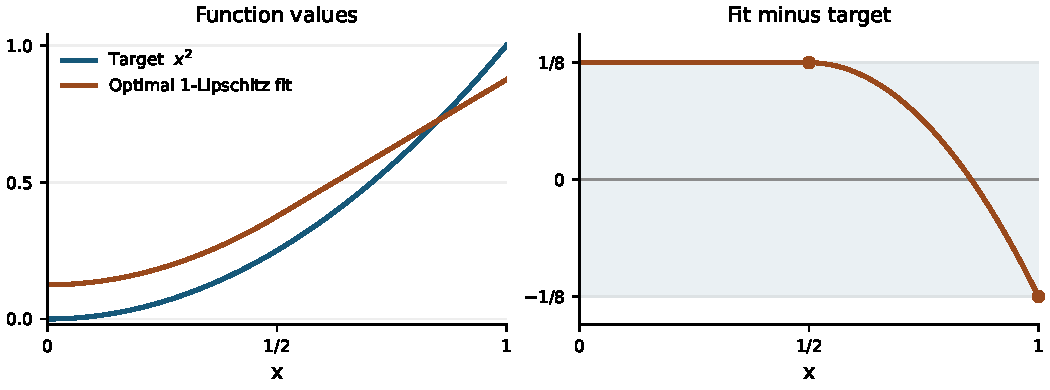
\includegraphics[width=.91\linewidth]{figures/variational.pdf}
\caption{At $L=1$, the optimal function meets its two extremal signed errors at $x=1/2$ and $x=1$. Those two evaluations already force the error $1/8$.}
\end{figure}

The finite-data analogue explains how the lower bound can be found. Suppose $u_i\in[0,1]\cap\Q$ are prescribed at a nonempty finite list of anchors $a_i\in D$. Put
\[
 e_*=\tfrac12\max_{i,j}\bigl(|u_i-u_j|-Ld(a_i,a_j)\bigr)_+.
\]
A fit of error $e$ at all anchors implies $|u_i-u_j|\le 2e+Ld(a_i,a_j)$, so $e\ge e_*$. To attain it, take the minimum of $1$ and the cones with heights $u_j+e_*$. Heights above one may be clipped to one, since their cones never lower that capped minimum. At $a_i$ the $i$-th cone gives the upper bound $u_i+e_*$. For every $j$, $u_j+e_*+Ld(a_i,a_j)\ge u_i-e_*$, and the cap is also at least $u_i-e_*$. Hence the error is at most $e_*$ and Lemma~\ref{lem:anchors} proves feasibility. Repeated anchor positions are allowed. This certificate explains why two opposed sample constraints determine the lower bound in the continuous example.

The file \texttt{Variational.lean} checks the rational lower bound, feasibility and attainment for arbitrary rational $0\le t\le1$ and every candidate $f:\Q\to\Q$ satisfying the interval guards. For real-valued named $f$ the lower-bound proof above uses the same rational inequalities with independent evaluation slack. The Lean quantifier over $f$ belongs to the metatheory. The object-language endpoint quantifies only over numerical parameters of a prescribed evaluator and its rational sample precision.

\subsection{An optimization over functionals}

There is a categorical reason the same answer survives a change of domain. Suppose $r:Y\to X$ and $s:X\to Y$ are nonexpansive maps with $r(s(x))=x$, and $u:X\to[0,1]$ is uniformly continuous. Call $e\ge0$ attainable if some $L$-Lipschitz $g:X\to[0,1]$ fits $u$ to uniform error at most $e$. Exactly the same tolerances are attainable on $Y$ for $u\circ r$. Indeed $g\circ r$ supplies the forward witness. For the converse, if $h$ fits $u\circ r$ on $Y$, the function $h\circ s$ fits $u$ on $X$ with the same error. Both composites preserve the Lipschitz constant. Whenever the infima are presented by our nets, these two witness transformations also give equal infima: apply them to the finite near-minimizers and let their prescribed errors decrease. An optimal witness on $X$ pulls back to an optimal witness on $Y$. Nonexpansiveness of both arrows controls the Lipschitz constant in these two transformations. The Lean theorem \texttt{fits\_retract} checks the witness equivalence on rational pseudometric carriers.

For an example in which the unknown is a functional, take $Y=\Lip_1([0,1],[0,1])$, $r(f)=f(1/2)$, and let $s(a)$ be the constant function $a$. Evaluation is nonexpansive in $f$; the uniform distance between two constant functions is exactly the distance of their values. The identity $r\circ s=\mathrm{id}$ is pointwise evaluation. Consequently
\[
 \inf_{\Phi\in\Lip_L(Y,[0,1])}\ \sup_{f\in Y}
       |\Phi(f)-f(1/2)^2|=\frac{(\max(0,2-L))^2}{8}.
\]
An optimal functional is $\Phi(f)=g(f(1/2))$ with $g$ from Theorem~\ref{thm:minimax}. All the constructions have algorithms on names: $r$ evaluates a cone name at the rational midpoint, while $s$ reads the scalar at the height precision and uses Theorem~\ref{thm:inner} to produce codes for the constant function. A single finite code need not encode an arbitrary constant exactly. On the lower-bound side only the constant functions of values $t$ and $1$ are needed. Thus the same two witnesses give the sharp answer even after two successive function-space constructions.

\section{Correspondences and continuous model theory}
\label{sec:metric-logic}

How much of a statement about a metric space survives if all we have is a
finite table of distances? The diameter survives a small uniform distortion
of the table. So does the radius, even though its definition alternates two
quantifiers. An entire fragment of continuous first-order logic survives with
the \emph{same} error as its atomic formulas. This gives both a way to evaluate
sentences and a way to refute a proposed identification of two spaces. The
quantifiers are the real-valued $\sup$ and $\inf$ of metric model theory.
We use a relational, bounded fragment of the semantics of Ben Yaacov,
Berenstein, Henson and Usvyatsov.%
\footnote{I.~Ben Yaacov, A.~Berenstein, C.~W.~Henson and A.~Usvyatsov,
\emph{Model theory for metric structures}, especially section~3.
\href{https://math.univ-lyon1.fr/~begnac/articles/mtfms.pdf}{Authors' text}.}

\subsection{A category of finite observations}

Fix a finite signature of relation symbols with declared arities, including
a binary symbol for distance. A stage $A$ has vertices $0,\ldots,a$, with
$a\geq0$, and a rational $[0,1]$-valued table $P_A$ for each symbol $P$.
A metric stage also requires the distance axioms, which are finite tests.
The transfer argument needs only the tables, so it applies to pseudometrics.
A correspondence of grade $e\geq0$ from $A$ to $B$ is a Boolean matrix $R$
in which every row and column contains a one. For each $k$-ary $P$ and each
$k$-tuple of paired vertices $x_i R y_i$, require
\[
  |P_A(x_1,\ldots,x_k)-P_B(y_1,\ldots,y_k)|\leq e.             \tag{C}
\]
For a nullary relation this tests its two values. The finite test loops over
at most $(|A||B|)^k$ tuples for $P$. Multiplying all rational entries,
constants and grades by a common positive denominator converts the
comparisons in a given instance to integer arithmetic.

If $A\xrightarrow{R,e} B\xrightarrow{S,d} C$, put
$x(SR)z$ when $xRy$ and $ySz$ for some $y\in B$. Search up to $|B|$
for the middle vertex. Successive uses of row coverage and of column
coverage prove both cover conditions. For paired tuples in $SR$, choose
the first witnessing middle vertex in each coordinate. Apply (C) to each
side and the triangle inequality to get grade $e+d$. The diagonal has
grade zero. In a triple composite both bracketings assert the existence of
the same two successive intermediate vertices, so their Boolean matrices
are equal. The diagonal laws follow by substituting its single forced
coordinate. Thus correspondences compose in a category, with upper
bounds on distortion that add under composition. The same arrow can have
several upper bounds.

This gives an instance of the repository's
\emph{PresentedCategory} interface. Use natural numbers for validated
stage and matrix codes, extensional equality of Boolean entries for
parallel arrows, and the bounded matrix product above. Omit the grade
from the arrow code and carry (C) as a predicate. Every two-sided covering
relation has grade one in the bounded signature. The existing
presentation-wise Yoneda calculation applies to this instance once
its coding laws have been internalized. Formula transfer uses the
additional quantitative information in (C).%
\footnote{ProveIt, under \nolinkurl{Derivations/Lean/IPRADerivations/Foundations},
\texttt{PresentedCategory.lean} and \texttt{Yoneda.lean}. Repository paths in
this section are relative to \nolinkurl{Logic/PrimitiveRecursiveArithmetic}.}

\subsection{Quantifier transfer with a depth-independent error}

Formulas are built from predicates on variable tuples and rational
constants in $[0,1]$ by $1-u$, $u\mathbin{\dot-}q=\max(0,u-q)$,
$\min(u,v)$, $\max(u,v)$, $\sup_x u$, and $\inf_x u$. On a stage,
the last two operations take the maximum and minimum over its vertices.
Every stage is nonempty. A closed formula thus has an exact rational
stage value $v_A(\varphi)$. An open formula has a value for each assignment
of its free variables.

\paragraph{Transfer theorem.}
If $R$ has grade $e$ and the two assignments agree along $R$ coordinate
by coordinate, then the two values of any such $\varphi$ differ by at most
$e$. This holds for every fixed formula and arbitrary encoded stages.

\begin{proof}
An atom gives precisely (C). A constant gives zero discrepancy. Reflection
around $1/2$ and truncated subtraction are 1-Lipschitz, as are minimum
and maximum on pairs with the maximum norm. For the last assertion, if
$u_i\leq v_i+e$ for $i=1,2$, monotonicity bounds the minimum (respectively
maximum) of the two $u_i$ by the corresponding extremum of the two $v_i$
plus $e$. Interchange the lists for the other inequality.

Suppose $\varphi=\sup_x\psi$. Select a maximizing vertex $x$ of $A$ by a
finite scan, then select $y$ from its row of $R$. The inductive assertion
bounds $\psi_A(x)$ by $\psi_B(y)+e$, hence by $\max_B\psi_B+e$.
A maximizer of $B$ and coverage of its column give the converse bound.
For $\inf_x\psi$, a minimizer of $A$ and row coverage give
$\min_B\psi_B\leq\min_A\psi_A+e$, and a minimizer of $B$ gives the converse.
Every binder inherits the same $e$ as its body. Row coverage alone only
gives one direction of each quantified estimate.
\end{proof}

The proof is a derivation scheme by external recursion on the fixed
formula. For a binder, the internal loop invariant records an index in
the scanned prefix, its evaluated value, and the fact that this value
dominates (or is dominated by) the prefix. This is a bounded Boolean
test. With the formula fixed, the evaluator and the relation test are PR
by nested bounded scans and composition. Variables are represented by
de Bruijn indices in a numerical tuple. Adding a binder shifts the old
indices and places the tested vertex at index zero. A proof for a new
connective requires an explicit modulus. For example
$\min(1,u+v)$ propagates two errors to $2e$. The depth-independent
constant in the theorem uses the displayed fragment.

\paragraph{A uniform arithmetic theorem for encoded formulas.}
For this finite grammar the scheme also admits a single formula-code
version. Give the syntax in postorder, with $h$ instruction rows and
all child indices smaller than their parent. Choose $K$ one above the
largest variable index in any atom, or zero if none occurs. Use integer
units with a positive common denominator $D$, and reject malformed
instructions, arities and constants by bounded tests. For a stage of
size $a$, allocate $h a^K$ table cells with entries in $[0,D]$.
Column $u<a^K$ is an assignment in base $a$ with $K$ digits, treating
$a=1$ as the unique all-zero assignment. For a binder, prepend a
vertex to the assignment and retain the first $K$ coordinates.
Take the maximum or minimum over the $a$ resulting child entries.
When $K=0$ there is just the empty assignment. An atom indexes its
predicate table, and all other instructions use at most two child
rows. Thus there is a uniform PR evaluator on formula and structure
codes. Its evaluation tables can be packed in base $D+1$ with bound
$(D+1)^{h a^K}$. These bounds express finite table evaluation even
for signatures that include an arbitrarily large numerical table.

For related stages of sizes $a,b$, induct on the number of rows filled.
The invariant says that in every completed row, entries in related
columns differ by at most $e$. Checking it costs a scan over at most
$h a^K b^K$ triples and $K$ matrix entries per column test. In a binder
row the selected extremum and the row or column witness produce a pair
of extended related assignments; that child row has already passed the
invariant. Each remaining row rule is one of the numerical inequalities
above. The empty prefix is vacuous. This is a single QF induction on
a Boolean equation and gives the code-uniform transfer theorem, also
for a postorder circuit which shares subformulas. It interprets each predicate by lookup in its bounded numerical table.

\paragraph{Arithmetical meaning of a model value.}
Suppose a fixed PR family of stages $A_n$ comes with verified matrices
from $A_n$ to $A_{n+1}$ of grades at most $2^{-n-1}$. For a sentence
$\varphi$ compute $v_n=v_{A_n}(\varphi)$. For $m\geq n$ transfer and finite
summation give
\[
 |v_n-v_m|\leq\sum_{j=n}^{m-1}2^{-j-1}=2^{-n}-2^{-m}.
\]
The summation uses QF induction on a cross-multiplied rational inequality
with the endpoint $n$ fixed. Hence $v_n$ names a real value with error at
most $2^{-n}$, even when the stages have different denominator grids.
Its upper cut at a rational $q$ can be observed strictly whenever
$v_n+2^{-n}<q$. The analogous lower test uses $q<v_n-2^{-n}$.
The zero condition is the arithmetic assertion
$\forall n\ (v_n\leq 2^{-n})$, by the tail bound and nonnegativity.
It need not be decidable. Strict tests on opposite sides cannot both pass,
and any positive margin eventually appears in a test by the geometric
error bound. A second presentation related at accuracy tending effectively
to zero yields the same cuts by the transfer theorem and these bounds.

\paragraph{When this evaluates an ordinary metric structure.}
Suppose a nonempty compact metric structure $M$ is supplied with finite
$r_n$-nets of actual sample points, $r_n\to0$ with a stated PR rate,
and evaluations of its atomic predicates at those samples with error
$\eta_n\to0$ of stated PR rate. Assume each predicate has a specified
Lipschitz bound $L_P$ for the maximum metric on its tuples. The distance
predicate has $L_d=2$. Let $L$ be the largest bound. Relate a point of
$M$ to each sample within $r_n$ of it. A sample is related to itself and
coverage supplies a sample for each point. The atomic discrepancy is at
most $e_n=Lr_n+\eta_n$. With this relation the preceding induction works
for ordinary suprema as well. For the upper bound on a supremum, bound
\emph{every} value on $M$ by the finite maximum plus $e_n$. For the
reverse, use a maximizing sample and its copy in $M$. The analogous
bounds for an infimum reverse the comparisons. This proof needs no
assumption that a supremum is attained in $M$.

Here is a constructive reading if those suprema have yet to be defined.
Induct externally through the formula. At a quantifier, finite extrema on
two nets agree to within $e_n+e_m$. Pair samples through a common point
of $M$, use net coverage in both directions and the atomic bounds on
both sides, and apply finite formula transfer. Its proof also applies to
this externally specified relation, which supplies witnesses for every
row and column. For free variables retain their common assigned points.
These extrema have a regular Cauchy name after applying the supplied
rates. Its upper-bound property for a supremum follows by approximating
each argument with a net point to arbitrarily small error. Its leastness
follows because every selected maximizing sample is itself a point of
$M$, where the already interpreted body has value within $e_n$ of the
sample evaluation. The dual proof gives infima. This proves the semantic
bridge for the supplied presentation. Inside iPRA the statements concern
numerical stage comparisons and cuts for fixed presented names. To apply
the bridge, a classical description still requires nets, evaluation
algorithms and moduli.

\paragraph{Constructing the comparison matrices.}
There is a direct numerical construction when distances between sample
points of different levels can also be approximated. Suppose a PR table
$\widehat d_{nm}$ approximates all such distances within $\tau$, and
each sample of either level has a covering witness on the other level
with the advertised net radius. Write $r=\max(r_n,r_m)$. Retain the
pair $(i,j)$ if $\widehat d_{nm}(i,j)\leq r+\tau$. Every supplied
covering pair passes. Every retained pair has true distance at most
$r+2\tau$. Consequently (C) holds with
\[
       e=\eta_n+\eta_m+L(r+2\tau).
\]
Each assertion is a bounded scan or a direct instantiation of a supplied
metric or predicate estimate. Thus we obtain the required Boolean
matrix even when exact comparison of a real distance with $r$ is
undecidable. For example, thin the levels by their PR rates so that
$r_n,\eta_n$ at the new index $j$ are at most
$2^{-j-4}/(L+1)$, using prefix maxima of requested indices if needed.
Compute cross-distances at that same accuracy for successive levels.
The displayed grade is at most $2^{-j-1}$, as required by the Cauchy
argument. This supplies a numerical bridge for named spaces with common
distance evaluation.

\subsection{A sentence separating two continua of the same diameter}

Let $I=[0,1]$ and let $T=\mathbb R/2\mathbb Z$ carry its shorter-arc
metric. Both have diameter $1$. Consider
\[
                    \rho=\inf_x\sup_y d(x,y).
\]
For $m\geq1$ use units $1/(2m)$. The interval stage consists of
$0,\ldots,2m$ with ordinary distance in integer units. The circle stage
consists of $0,\ldots,4m-1$, with
$d(i,j)=\min(|i-j|,4m-|i-j|)$. Each point is within $1/(2m)$ of a
sample, and all sample distances are exact. For a constructive name
a rational approximation finer than one quarter of the mesh and rounding
it to a nearest sample give an explicit covering witness, including at a
circle seam by reduction modulo $4m$.
At an interval vertex $i$ the farther endpoint is at distance at least
$m$, while all vertices are within $m$ of the midpoint $m$.
At every circle vertex its antipode has distance $2m$, and no distance
exceeds $2m$. Thus the normalized interval and circle values are
$1/2$ and $1$ at every stage. The net bridge gives those same values
on the continua. Any proposed correspondence between these grids has
distortion at least $1/2$ even with arbitrarily fine mesh. The same
obstruction holds for a two-sided correspondence on the continua with
uniform distance distortion, by the supremum/infimum inequalities in
the transfer proof.

\subsection{Descent with a stated overlap error}

The repository's categorical methods paper proves exact gluing and
explicitly flags the missing error estimate for approximate overlap
data.%
\footnote{ProveIt, \nolinkurl{docs/proofs/foundations/ipra_categorical_methods/paper/sections/05_descent.tex},
subsection on a finite sheaf of function tables.}
Let a finite source stage $X$ be covered by masks $U_i$.
At each $x\in U_i$ there is a value $f_i(x)$ in a rational
pseudometric table $Y$. On overlaps assume
$d(f_i(x),f_j(x))\leq e$. Inside a patch, suppose a specified symmetric
nearness test $N(x,y)$ implies $d(f_i(x),f_i(y))\leq w$
when both points are in $U_i$. Finally require the finite cover
condition that every $N$-near pair lies in some common patch.

Choose the first patch $s(x)$ containing $x$, and set
$g(x)=f_{s(x)}(x)$. Every local value at $x$ is within $e$ of $g(x)$,
so every two patch selectors agree to within $e$. For any $N$-near
pair choose a common patch $i$. The three successive comparisons
\[
 g(x),\quad f_i(x),\quad f_i(y),\quad g(y)
\]
have costs $e,w,e$, so $d(g(x),g(y))\leq2e+w$. Any other global
table within $e$ of every patch is within $e$ of this particular selector
at each point, and two arbitrary such tables are within $2e$ of one
another. The $2e+w$ bound for arbitrary selectors is sharp with two singleton
patches followed by a two-point common patch. Take the common-patch
values $e,e+w$ in the rational line and the singleton values $0,2e+w$,
respectively. The first-cover selector takes both extreme values.
Rescale if a unit-diameter target is desired.

All hypotheses, including the common-patch condition, can be tested by
bounded table scans. Without the common-patch condition two nearby
points in disjoint singleton patches can be assigned unrelated values
even when $e=w=0$. A continuous application requires these estimates on
a refining family with accuracy tending to zero and coherence between
its selected global tables. For example, if matched vertices on two
levels admit corresponding patches whose local values agree within
$c$ in a common target, then their selected global values differ by at most
$e_n+c+e_{n+1}$, by the same three comparisons. With a summable PR
bound and PR tail modulus on these successive discrepancies one obtains
Cauchy names along specified compatible vertex names.

\begingroup\setlength{\emergencystretch}{3em}
\paragraph{Formalization.}
In \texttt{lean/Abstract.lean}, the correspondence laws underpin
\texttt{formula\_\allowbreak transport}. The calculations of both radii give
\texttt{circle\_\allowbreak line\_\allowbreak obstruction}, and the patch estimate is
\texttt{glue\_\allowbreak oscillation}. Its truth values and errors are integer units,
so arbitrary rational finite instances use one common denominator. The
file quantifies over Lean functions to state reusable lemmas. For a literal
object-theory derivation, instantiate the vertex sets by bounds, encode
each relation by a Boolean matrix and each predicate by its table,
totalizing malformed accesses by zero. The maximum/minimum loop needs
the extremum index and the bounded prefix domination test described
above. Relate variable assignments by a bounded conjunction over the
free positions. Derive the two quantifier inequalities by those extremum
indices and the two covering scans, then compile connective cases by
substitution. This produces an object proof for each fixed formula. The preceding postorder invariant gives the alternative route for one theorem over formula codes.
The Lean file checks the reusable semantic proof and the exact grid
calculation. The table-code compiler and its object-proof output for
this complete fragment remain to be mechanized.
\par\endgroup

\section{A nerve theorem with constructed homotopies}
\label{sec:boxnerve}

The ProveIt topology report leaves open an effective nerve theorem with
produced contraction data (\href{https://github.com/VladimirReshetnikov/ProveIt/blob/5f3be02388442f16487d2dc5c2529961dd783d2b/Logic/PrimitiveRecursiveArithmetic/docs/proofs/topology/ipra_topology_framework_2026-11-15/paper/sections/12_limits.tex}{topology report, residual obligations}). Here is a case in which the input consists
entirely of coordinates. It includes spaces with holes, disconnected
spaces, boxes of dimension less than the ambient dimension, and
intersections with zero clearance. The classical closed convex nerve
theorem and the forward map from a subdivided nerve are well established
(Bauer, Kerber, Roll and Rolle, \emph{Expositiones Mathematicae}, 2023,
\href{https://doi.org/10.1016/j.exmath.2023.04.005}{doi:10.1016/j.exmath.2023.04.005}).
The issue here is the arithmetic cost of constructing both homotopies,
particularly near a boundary shared by several boxes.

\paragraph{The statement.}
Let $B_1,\ldots,B_m$ be nonempty closed axis-parallel rational boxes in
$\mathbb R^d$, with $m\geq1$. Write $U=\bigcup_i B_i$ and let $N$ have a
nonempty face $J\subseteq\{1,\ldots,m\}$ precisely when
$\bigcap_{i\in J} B_i\ne\varnothing$. Realize $|N|$ in the probability
simplex by requiring the support of a point to be a face. Use the maximum
norm on both spaces. On finite rational data there are primitive recursive
constructions of maps
\[
 F:U\longrightarrow |N|,\qquad G:|N|\longrightarrow U
\]
and homotopies from the identities to $GF$ and $FG$. The constructions
supply rational Lipschitz bounds for every map and homotopy. They extend
to regular Cauchy names. An inclusion of covers taking each box into a specified
target box commutes with $G$ up to a constructed homotopy. An empty
family can be handled separately by the empty nerve and the empty union.

\paragraph{Finite presentations.}
Write $B_i=\prod_j[\ell_{ij},u_{ij}]$. For nonempty $J$, compute
$L_j(J)=\max_{i\in J}\ell_{ij}$ and
$V_j(J)=\min_{i\in J}u_{ij}$. Testing $L_j\leq V_j$ for every $j$
decides the nerve table, including tangencies. A positive result gives
the point $p_J=(L_j(J))_j$ and the contraction to $p_J$ by linear
interpolation in the intersection.

Cut the bounding rectangle $R$ by all box endpoints in each coordinate.
The factors of a grid face are knots or closed intervals between successive
knots. Retain every face $c$ contained in at least one $B_i$. These faces
form a cubical complex $K$ with realization $U$. Indeed each box and all
its faces are unions of grid faces. Set $I(c)=\{i:c\subseteq B_i\}$.
This is a nerve face, since the center of $c$ belongs to all its boxes.
Inclusion of grid faces reverses inclusion of their index sets. The grid
has at most $(4m-1)^d$ nonempty faces before restriction and $N$ has at most
$2^m-1$ nonempty faces. Each coordinate with a single knot is kept constant.

For any nonempty face $J$ of the probability simplex let $b_J$ have value
$1/|J|$ on $J$ and zero elsewhere. Barycentric subdivision of the grid has
a simplex for each strict chain $c_0\subsetneq\cdots\subsetneq c_s$,
with vertices the centers $b(c_j)$ of these faces. To see directly that it
covers a box face, join its center to the subdivision of its boundary.
Every point other than the center lies on a unique radial ray from the
center to that boundary. Repeating on faces gives a convex combination of
centers down to dimension zero. The subdivisions on common faces agree.
For the probability simplex there is an equally explicit description.
Sort the distinct positive coordinate values $v_1>\cdots>v_k>0$, set
$v_{k+1}=0$, and use $J_a=\{i:y_i\geq v_a\}$.
The coefficient of $b_{J_a}$ is $|J_a|(v_a-v_{a+1})$. These nonnegative
coefficients sum to one and telescope in each coordinate.
Coincident values introduce a zero coefficient in a sorted enumeration.
No choice on a shared boundary affects the interpolation.

\paragraph{The two maps.}
On a subdivided grid vertex put $F(b(c))=b_{I(c)}$. Extend affinely along
each chain. Its images are a chain of barycenters of nerve faces in reverse
order, with possible repetitions. Hence $F(x)\in |N|$.
Put $G(b_J)=p_J$ and extend affinely on each subdivided nerve simplex.
For a chain $J_0\subsetneq\cdots\subsetneq J_k$, all its selected points
belong to each $B_i$ for $i\in J_0$. Convexity gives the same containment
for $G(y)$. Affine formulas agree on faces in both constructions.

For $x$ in a grid chain ending at $c_s$, choose any $i\in I(c_s)$.
The point $x$ lies in $B_i$. Every $I(c_j)$ contains $i$, so
$p_{I(c_j)}\in B_i$. Since $G$ is affine on the chain of the $I(c_j)$,
$GF(x)$ is the combination of these latter points with the original
weights. Thus $(1-t)x+tGF(x)$ stays in $B_i$ for $0\leq t\leq1$.

\paragraph{The homotopy on the nerve.}
Fix a rational $y$ with its positive-weight chain
$J_0\subsetneq\cdots\subsetneq J_k$. Choose $i\in J_0$. Every barycenter
in this chain has $i$-coordinate at least $1/m$. Thus $y_i\geq1/m$.
The point $G(y)$ belongs to $B_i$. More generally, whenever $x\in B_i$,
the largest grid face with positive weight in its subdivided presentation
is contained in $B_i$. Indeed $x$ lies in the relative interior of that
face, because its center has positive weight. A box with grid endpoints
containing such a point contains the entire face. Every smaller face
in the chain is contained as well. Consequently $F(x)_i\geq1/m$.
Taking $x=G(y)$ gives a coordinate shared with quantitative mass:
\[
  y_i\geq1/m,\qquad (FG(y))_i\geq1/m.
\]
The calculation of the homotopy does not require the index $i$.
Write $v=FG(y)$ and define
\[
   z_j=\min(y_j,v_j),\qquad S=\sum_j z_j\geq1/m,\qquad P(y)=z/S.
\]
The support of $P(y)$ lies in both supports. Travel along the segment
from $y$ to $P(y)$ during the first half of the unit interval and along
the segment from $P(y)$ to $v$ during the second half. Each segment lies
in a single nerve simplex. The midpoint formulas agree. This construction
gives a global formula using only rational operations and a guarded
reciprocal. It also works when the direct segment from $y$ to $v$ leaves
the nerve.

\paragraph{Continuity and proof strength.}
Here are bounds that do not presume a Lebesgue number for the input.
Extend the vertex formula for $F$ to every grid face in $R$, assigning
$e_1$ whenever $I(c)$ is empty. Extend $G$ to the entire probability
simplex, assigning $p_{\{1\}}$ on barycenters of nonfaces. Their affine
extensions still land in the full simplex and in $R$, respectively.
Compute the affine matrices of the finitely many full-dimensional pieces
by solving their rational vertex equations. Constant domain coordinates
are dropped, and for the probability simplex the last coordinate is
dropped. The latter projection is $1$-Lipschitz into the coordinate
chart with maximum norm. In dimension zero the linear part is zero.
The largest absolute row sum over all pieces is a Lipschitz bound on a
convex domain: a rational segment can be cut at its intersections with
the finite affine walls, and the lengths of its collinear pieces sum to
the segment length. If a segment lies on a wall the two adjacent affine
formulas agree there. Thus the two computed bounds $L_F,L_G$ work even
for pairs lying in distinct components of the original domain.
The determinant algorithm may use the bounded permutation formula.

Set $D=L_FL_G$ and $L=\max(1,D)$. The first homotopy has Lipschitz bound
$L+\operatorname{diam}_\infty R$ on the product with time, using the maximum
product metric. For the second, $z$ is $L$-Lipschitz and $S$ is
$mL$-Lipschitz. Comparing $z_j/S$ with $z'_j/S'$ and using
$z'_j/S'\leq1$ bounds the change by
$m(|z_j-z'_j|+|S-S'|)$. Thus $P$ is $m(1+m)L$-Lipschitz on $|N|$.
Interpolating in time costs at most $2$, so $m(1+m)L+2$ suffices for
the second homotopy. If an evaluator has bound $A$, an input known to
accuracy $2^{-(k+\lceil A\rceil+1)}$ gives output error below $2^{-k}$.
This intentionally coarse shift avoids logarithms.

Internally, use rational points of $U$ and $|N|$ as dense presentations
and code all regular names via their rational observations. An input
approximation on either side is required to belong to the presented
rational space. Rational cell location is decidable, and common-face
agreement and the Lipschitz bounds make the output independent of
approximants. Externally, the resulting maps extend to the metric
completions; in ordinary real geometry these are exactly the indicated
closed polyhedra. This distinction avoids a case decision on an exact
real at a box face. All statements about pointwise errors reduce to
cleared rational inequalities. To implement the two subdivisions,
enumerate chains of length at most $d+1$ for the grid or $m$ for the
nerve, discard dependent candidates by a determinant test and test
barycentric coefficients by sign and summation. Lower-dimensional
chains use any nonsingular minor of the right size and check all ambient
equations. Include the singleton case. All scans are bounded by the
face counts above raised to the corresponding chain lengths, up to
summing over lengths; each coordinate scan and each permutation sum has
its own finite bound. Existence of a containing simplex follows from
the radial decomposition with at most $d$ strict dimension drops or
from the sorted-coordinate formula with at most $m$ steps. At a grid
face $[a,b]$, the radial step divides by the largest of the absolute
rescaled coordinates $|2(x_j-a_j)/(b_j-a_j)-1|$ over nonconstant
coordinates, after testing the center case. Rational comparison guards
this division.

A quantifier-free induction for the weighted-coordinate estimate keeps
a partial numerator and the corresponding sum of weights. The invariant
after $r$ terms is
$m\sum_{j<r}w_j a_j\geq D_0\sum_{j<r}w_j$, where coordinates have
common denominator $D_0$ and $m a_j\geq D_0$. The next inequality follows
by multiplication by $w_r$ and addition. The mass bound uses the
one summand belonging to the common coordinate. Grid tests, incidence
checks, membership of a running intersection, and agreement of two
affine pieces at the vertices of their common face are finite Boolean
folds. On a fixed rational segment the partition at affine walls has
at most two endpoints per simplex in a brute-force implementation:
intersection of a simplex with a line segment is an interval whose
endpoints follow from its rational barycentric inequalities. Sorting
these rational parameters and summing the Lipschitz estimates is
another quantifier-free prefix invariant. The capacity bounds above
are primitive recursive in the input, including the dimension.

\paragraph{Naturality for inclusions and an exact persistence interval.}
Suppose $B_i\subseteq C_{r(i)}$ for a finite index map $r$. Let
$r_*$ send each subdivided vertex $b_J$ to $b_{r(J)}$ and be affine on
chains. Taking images of finite subsets commutes with composition,
including collapsed faces. For $y$ in a chain beginning at $J_0$,
pick $i\in J_0$. Both $G_B(y)$ and $G_C(r_*y)$ are in $C_{r(i)}$.
The straight homotopy in that box proves commutation up to homotopy.
The usual linear nerve map and $r_*$ are likewise joined by straight
segments: on a chain ending at $J_k$ both lie in the simplex $r(J_k)$.
All these arguments work at face contacts.
Consequently in the usual homology interpretation the nerve isomorphisms
respect the maps of a filtration. This uses ordinary homotopy invariance
as a semantic consequence; the finite arithmetic output consists of the
maps, homotopies, and their budgets.

For instance, take the bottom, right, top and left bars
\[
 [0,3]\times[0,1],\quad [2,3]\times[0,3],\quad
 [0,3]\times[2,3],\quad [0,1]\times[0,3]
\]
in that order. At $y=(3/4,1/4,0,0)$ the subdivided weights on
$\{1\},\{1,2\}$ are both $1/2$. Thus $G(y)=(1,0)$,
$FG(y)=(1/2,0,0,1/2)$, $S=1/2$ and $P(y)=e_1$.
The union of the two endpoint supports contains the disjoint left and
right bars. A single straight homotopy between those endpoints would
leave the nerve (Figure~\ref{fig:boxnerve}).
\begin{figure}[htbp]
  \centering
  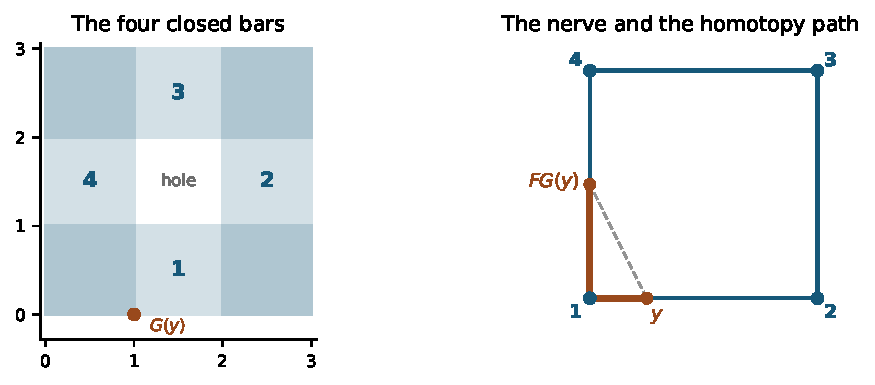
\includegraphics[width=.86\linewidth]{figures/box_nerve.pdf}
  \caption{The four bars and their nerve at $t=0$. The orange path passes
  through vertex $1$. The dashed chord crosses the missing simplex.}
  \label{fig:boxnerve}
\end{figure}
Now thicken all bars in the maximum norm by $t\geq0$.
For $t<1/2$ consecutive bars meet and opposite ones are disjoint, so
the nerve is exactly a four-cycle. For $t\geq1/2$, $(3/2,3/2)$ belongs
to all four, so the nerve is the full tetrahedron. Inclusion before the
threshold induces the identity on the four labels. Over $\mathbb F_2$,
the only nonzero $1$-cycle in the four-cycle is the sum of its four
edges, since even incidence at every vertex forces all coefficients to
coincide. There are no triangles. In the full simplex every $1$-cycle
bounds: cone its edges to vertex $1$, omitting repeated-vertex
triangles; the terms from incident endpoints cancel by even incidence.
Hence this filtration has exactly one degree-one interval $[0,1/2)$.
Rational $t$ already gives its entire finite-arithmetic statement.
The exact evaluator in \texttt{examples/box\_nerve.py} reproduces these
intersections, both maps at the specified point, and the overlap mass.

\paragraph{Lean path.}
\texttt{lean/Topology.lean} proves the intersection fold, lower-corner
criterion, weighted-coordinate lower bound, support of a minimum, and
the overlap denominator estimate after clearing denominators. Its
\texttt{overlap\_segments} theorem constructs the two segments at rational
parameters: blending $x/D$ and $z/S$ with time $b/(a+b)$ gives numerators
$aS x_j+bD z_j$ with total $(a+b)DS$. It proves the corresponding total
and valid support on both halves.
To finish the spatial layer, code an axis face by a knot or an interval
index and use face chains with rational barycentric weights. Prove the
radial-step reconstruction by clearing its tested denominator, then
induct on the number of nonconstant coordinates. Prove reconstruction
of the simplex coordinates by telescoping sorted differences. On these
witnesses the two interpolation maps are finite weighted sums.
Composing the two chain maps on the grid side only merges repeated
index sets, preserving those sums. On the nerve side apply
\texttt{weighted\_lower} twice to the common-index argument and
\texttt{overlap\_mass} once before dividing. The remaining estimates are
the affine matrix calculation and rational segment subdivision above.
Quoting these finite kernels into the repository calculus remains a
separate derivation task. Arbitrary convex bodies given by membership
oracles would require additional procedures for producing their
intersection witnesses and a compatible subdivision.

\section{Residues at constructively named complex points}
\label{sec:movingres}

The repository's \href{https://github.com/VladimirReshetnikov/ProveIt/blob/5f3be02388442f16487d2dc5c2529961dd783d2b/Logic/PrimitiveRecursiveArithmetic/docs/proofs/analysis/cauchy_residue_ipra/report.tex}{Cauchy and residue report}
builds Laurent coefficients at rational singularity centres. Its final section on curves retains this restriction. We remove it for a finite list of positively isolated centres given by regular PR names. The issue is that substituting a nonrational centre changes the domain on which the function can be sampled. Using one fixed rational collar for all sufficiently accurate approximations gives an explicit solution.

Write $|u|_1=|\Re u|+|\Im u|$, $|u|_\infty=\max(|\Re u|,|\Im u|)$, and $Q_t(b)=\{z:|z-b|_\infty\le t\}$ for a closed square oriented counterclockwise on its boundary. A centre name $A(n)\in\mathbb Q(i)$ satisfies
$|A(n)-A(m)|_1\le 2^{-n}+2^{-m}$. The letter $a$ denotes this name in completed-space notation. For $u\ge0$ write $s(u)$ for the least $t\le 1+\lceil u\rceil$ with $2^t\ge\max(1,u)$. This is a bounded PR search.

\subsection{Two finite tools and the rational input theorem}

Suppose two edge sums use identical increments $h_i$ and respective integrand samples $v_i,v_i'$, with $|v_i-v_i'|_1\le d$. Their difference has norm at most
\begin{equation}
 \left|\sum_{i<N}(v_i-v'_i)h_i\right|_1
 \le d\sum_{i<N}|h_i|_1. \label{eq:ccquad}
\end{equation}
Indeed $|uv|_1\le |u|_1|v|_1$ on expanding the two real coordinates. Apply the triangle inequality to each additional term. This proves the estimate at every finite refinement, at the cost of the contour length alone. For trapezoidal quadrature, use the average of the two endpoint samples on each panel. The same proof applies.

For two corresponding sides $[u,v]$, $[U,V]$ of squares with the same half-side, take the triangles $(u,v,V)$ and $(u,V,U)$. Their boundaries sum to
$[u,v]-[U,V]+[v,V]-[u,U]$. Over the four sides the connecting edges cancel. The signed identity holds also when two of the vertices coincide or a strip has zero area. Thus eight triangles join the two boundaries. Integrals are additive under splitting an edge, as follows by comparing both quadratures on a common refinement.

We use two quantitative lemmas from the linked report, its sections on uniform triangle subdivision and on annular Laurent expansion. Their input is a rational carrier with fixed PR evaluators for $f,f'$ at rational arguments, sample errors $2^{-n}$, bounds and uniform moduli. In name notation their operative conditions are
\[
 \begin{aligned}
 |u-v|_1\le2^{-\nu(k)}&\quad\Longrightarrow\quad |f(u)-f(v)|_1\le2^{-k},\\
 |u-v|_1\le2^{-\mu(k)}&\quad\Longrightarrow\quad
 |f(v)-f(u)-f'(u)(v-u)|_1\le2^{-k}|v-u|_1.
 \end{aligned}
\]
In finite form the first conclusion has the two sample errors added. The second, with all three evaluations at precision $n$, has the additional error $(2+|v-u|_1)2^{-n}$. We take the moduli nondecreasing using bounded maxima.

The first lemma gives zero integral on the boundary of a rational triangle contained in the carrier. At subdivision depth $m$, an affine first-order approximant integrates to zero around each child. Its error on that child is bounded by its diameter times $2^{-k}$ times its perimeter. There are $4^m$ children, each diameter and perimeter scaling by $2^{-m}$. The exact shared-edge cancellations leave a bound $DP2^{-k}+P2^{-n}(2^{m+1}+D)$ at sample precision $n$, for parent diameter $D$, perimeter $P$, and $D2^{-m}\le2^{-\mu(k)}$. All three indices can therefore be chosen by bounded arithmetic at the requested precision.

The second lemma treats a rational origin and the radii $s_0=r/8$, $R=8r$. A function $g$ on $Q_R(0)\setminus\operatorname{int}Q_{s_0}(0)$ bounded by $M$ has coefficients
\[
 c_\ell(g)=\frac{1}{2\pi i}\int_{\partial Q_t(0)}g(u)u^{-\ell-1}\,du,
 \qquad t=R\ (\ell\ge0),\quad t=s_0\ (\ell<0).
\]
On $\partial Q_r(0)$ the truncation from $-N$ through $N-1$ has error at most
$C2^{-N}$, with $C=16RM/(R-r)+16s_0M/(r-s_0)$. In particular $\int_{\partial Q_r(0)} g=2\pi i c_{-1}(g)$. To recall the origin of the margin, removing a small square about the evaluated point from the annulus and applying triangle cancellation gives the annular Cauchy formula. On the outer contour $|z/u|_1\le1/2$, and on the inner $|u/z|_1\le1/2$. Expanding each kernel by the exact finite geometric identity leaves the displayed uniform tail. Integrating monomials around a square extracts the $-1$ term. The report proves the kernel moment and quadrature bounds. We invoke these human-level arithmetic proofs as prior lemmas. Their deep Lean derivations are additional dependencies.

\subsection{Transport theorem}

For each centre choose a positive rational $r$ and $n_0$ such that $2^{1-n_0}\le r/32$, and take $b=A(n_0)$. One may take $n_0=1+s(32/r)$. Require effective holomorphy data as above on the rational closed collar
\[
 K(b,r)=\{v:r/16\le |v-b|_\infty\le 9r\}.
\]
Such collars are finite rational polygonal carriers. For a finite rational polygonal cycle $\Gamma$ assume there is a rational triangle chain $T$ and integer weights $w_j$ with
\[
 \partial T=\Gamma-\sum_j w_j\partial Q_{r_j}(b_j).
\]
Use one compatible $f$ on all these carriers, with effective holomorphy data on the triangles of $T$. For the winding interpretation assume disjoint proxy squares and that $T$ and $\Gamma$ avoid the open cores $|z-b_j|_\infty<r_j/16$. Equality after splitting rational edges, disjointness and clearance are finite geometric conditions. A common PR evaluator in the centre index and precision is required if the length of the family varies in the object formula.

\paragraph{Theorem.} On each translated annulus the Laurent coefficients about the named centre have PR names. On its middle square the same $C2^{-N}$ truncation bound holds. If $c_{j,-1}$ denotes the coefficient so obtained, then
\[
             \int_\Gamma f(z)\,dz=2\pi i\sum_j w_j c_{j,-1}.
\]
The weights agree with the winding numbers at the named centres under the clearance conditions above. If the presentation extends compatibly throughout a positively isolated punctured neighbourhood of each centre, $c_{j,-1}$ is its residue. The statement includes essential isolated singularities whenever these data are supplied.

\paragraph{Proof.} Fix one centre. For $n\ge n_0$ put $g_n(u)=f(A(n)+u)$ on the fixed annulus about zero. Its rational sample positions all lie in $K(b,r)$ because the displacement from $b$ has norm at most $r/32$ and
$r/8-r/32\ge r/16$, $8r+r/32\le9r$. The same translation in both arguments preserves their difference exactly. The bounds, function modulus and derivative remainder modulus of every $g_n$ are therefore identical. Apply the rational annular lemma at every stage, obtaining $c_{n,\ell}$ and one common $C$. Each $c_{n,\ell}$ here is already a name produced by a fixed quadrature algorithm with numeric parameters $n,\ell$.

For $n,m\ge\max(n_0,\nu(k)+1)$ and any rational $u$ on the annulus,
$|g_n(u)-g_m(u)|_1\le2^{-k}$. Both arguments lie in the collar and their distance is at most $2^{1-\min(n,m)}$. To name the translated value at precision $p$, take this index bound with $k=p+2$ and evaluate $F(A(n)+u,p+2)$. The translation and evaluation errors are each at most $2^{-p-2}$. Coherence at any two requests follows by comparison at a common finer stage.

Now compare the two coefficient quadratures on the same square about zero. Its kernel $u^{-\ell-1}$ has the same value at both sampling points in the reference coordinates. Put
\[
 H_\ell=
 \begin{cases}
  8R\max(1,2/R)^{\ell+1}, & \ell\ge0,\\
  8s_0\max(1,2s_0)^{-\ell-1},&\ell<0.
 \end{cases}
\]
Indeed $|u^{-1}|_1\le 2/|u|_\infty$ and $|u|_1\le2|u|_\infty$. The reciprocal of $2\pi i$ has norm less than one. Estimate~\eqref{eq:ccquad}, followed by arbitrary common-refinement accuracy, yields
$|c_{n,\ell}-c_{m,\ell}|_1\le H_\ell 2^{-k}$.
For a rational name of $c_\ell$ at precision $p$, take
$k=p+2+s(H_\ell)$,
$n=\max(n_0,\nu(k)+1)$, and evaluate $c_{n,\ell}$ to $2^{-p-2}$. This diagonal is PR jointly in the signed index and precision. It depends extensionally on the centre since two equal regular names become arbitrarily close with the same dyadic shifts (compare via a common finer stage). No modulus for the variation of $f'$ as the centre moves has been used.

To transfer the Laurent estimate, first fix $N$ and a rational $u$ on $\partial Q_r(0)$. A perturbation bounded by $\eta$ in each of the $2N$ coefficients changes the polynomial by at most $2N\max(1,2r,2/r)^N\eta$. Thus for an auxiliary tolerance $2^{-p}$ one can take the maximum of the explicit $n$ schedules for the finitely many coefficients with precision $p+2+s(2N\max(1,2r,2/r)^N)$ and the value schedule for $g(u)$. The rational inequality then holds with error $C2^{-N}$ plus arbitrarily small dyadic slack. Positive rational gaps are decidable and are separated from zero by an explicit reciprocal-denominator bound. This removes the slack in the name inequality. The same argument on smaller bands gives the Laurent germ wherever the rational annular estimate gives one. For compatible punctured-neighbourhood data, compare any two such radii on an intervening closed annulus. Translation to a sufficiently accurate common rational centre puts both radii in its supplied collar data (use a finite chain of overlapping closed bands with slack if needed). Triangle cancellation for the weighted integrand makes the coefficients equal there, and the preceding estimate passes that equality to the names. Here the punctured-neighbourhood input includes such working data for every pair of dyadic scales, uniformly in the scales. A single annular presentation by itself determines only its annular coefficient.

Finally join $\partial Q_r(b)$ to $\partial Q_r(A(n))$ by the eight rational triangles above. Every point in these triangles is a side point of the reference square plus a displacement of norm at most $r/32$ from $b$. Each pair of sides spans a parallelogram, including degenerate ones. Its infinity-distance from $b$ lies between $r-r/32$ and $r+r/32$. Cauchy's triangle lemma gives equal integrals. At the other end, the rational annular lemma gives $2\pi i c_{n,-1}$. Applying triangle cancellation on $T$ and taking the directed accuracy just proved gives the asserted formula. Explicitly, errors $\eta$ in the coefficients cost at most $8\eta\sum_j|w_j|$ since $2\pi<8$. The integral, product and constants receive their own dyadic sample margins. The straight segment from $b_j$ to any sufficiently accurate $A_j(n)$ lies in its empty core. At these rational points the oriented boundary of each triangle in $T$ has winding zero, the $j$th proxy square has winding one and the other squares have winding zero. Equivalently one may use the report's rational crossing algorithm. This stable value defines the winding at the named point. No comparison of a named coordinate for equality with a ray or vertex is required.\hfill$\square$

\paragraph{A nonrational two-coordinate pole.}
Let $a=(\sqrt 2+i\sqrt 3)/8$ and
$f(z)=(1+i)/(z-a)+1/(z-a)^2$. The centre approximation divides
$\lfloor\sqrt{2\,4^n}\rfloor+i\lfloor\sqrt{3\,4^n}\rfloor$ by $8\cdot2^n$. Integer square root is bounded search, and its two coordinate errors sum to less than $2^{-n}/4$. Use $r=1$, $n_0=6$, $b=(90+110i)/512$, and $\Gamma=\partial Q_2(b)$. Eight triangles fill the gap between $\Gamma$ and $\partial Q_1(b)$, using the four corresponding outer and inner sides. On $K(b,1)$ we have $|z-a|_\infty\ge1/32$, hence $|(z-a)^{-1}|_1\le64$. For a bound $U$ on the endpoint inverses, their difference is at most $U^2|h|_1$ and the inverse's linearization error at increment $h$ is at most $U^3|h|_1^2$, by the exact reciprocal difference identity. Squaring the inverse gives a remainder bounded by $3U^4|h|_1^2$ (expand $(v+\Delta)^2$ and use $|\Delta|_1\le U^2|h|_1$). Thus $M=2U+U^2$, a Lipschitz bound $L=2U^2+2U^3$ and a quadratic remainder constant $2U^3+3U^4$ provide the required inputs. A rational integrand sample is obtained using $A(n)$ at a precision shifted by $s(L)+2$ and enough initial bits to keep the inverse bound. For $n\ge6$ the same bound $64$ holds relative to $b$ for those proxies. Its polynomial derivative uses the same bounded inverse and finite products and therefore also has a PR name. Direct expansion about $a$ gives the residue $1+i$ and the integral $2\pi i(1+i)$.

The supplied \texttt{examples/moving\_pole.py} checks this example by independent midpoint quadrature along $\Gamma$. Here $|z-A(n)|_\infty\ge63/32$ for $n\ge6$, so $U=2$ and $L=24$ suffice on the contour. With $2^{14}$ panels per side, centre precision $20$, and $24$ bits after the binary point in each integrand coordinate, a taxicab error bound is
\[
 16\left(24\cdot2/2^{14}+24/(4\cdot2^{20})+2/2^{24}\right)
 =24625/524288<0.047 .
\]
The program compares with independent rational upper and lower sums for $2\pi=8\int_0^1(1+x^2)^{-1}dx$. All its comparisons use integers and fractions.

\paragraph{An essential singularity at the same point.}
Take $f(z)=\exp(1/(z-a))$ with the same squares. Here are explicit contracts to instantiate the result. For an integer inverse bound $U\ge1$ set $J=2U$, $t_j=U^j/j!$ and $B=\sum_{j<J}t_j+2t_J$. Beyond $J$ the ratio of consecutive terms is at most $1/2$, so every partial tail starting at $N\ge J$ is at most $2t_J2^{-(N-J)}$. The polynomial approximants to the exponential and its derivative therefore have PR rates and norm bound $B$ on $|v|_1\le U$. For $|v|_1,|w|_1\le U$, telescoping the powers twice bounds the $j$th monomial's first-order remainder by $\binom j2 U^{j-2}|w-v|_1^2$ for $j\ge2$. After division by $j!$ and summation the bound is $(B/2)|w-v|_1^2$. Composing with the reciprocal gives Lipschitz constant $BU^2$ and quadratic remainder constant $B(U^3+U^4/2)$ on the collar. Take $U=64$ here and enlarge it by the explicit reciprocal clearance on any smaller admissible annulus. The same series is already a uniformly convergent Laurent expansion in $z-a$, with every coefficient of $(z-a)^{-n}$ equal to $1/n!$ for $n\ge1$. Square moments give uniqueness coefficient by coefficient. This verifies both a residue of $1$ and an unbounded principal part, using the explicit tail bound at each requested precision.

\paragraph{Formalization boundary.}
The file \texttt{Complex.lean} proves both finite tools in Lean's ordinary arithmetic. The theorem \texttt{same\_increments} controls quadrature error for Gaussian rationals, and \texttt{four\_strips} gives the boundary identity. The theorem \texttt{diagonal\_regular} also verifies the two-level name construction, taking the sample at stage $\operatorname{cut}(p+2)$ and inner precision $p+2$ once the outer coefficient error has been normalized to $2^{-p}$. To construct the object proof, encode the signed fractions, point samples and edges as natural numbers, clear positive denominators and use the fixed-precision prefix inequality in~\eqref{eq:ccquad} as the QF induction invariant. Include a Boolean fold of the finite sample hypotheses. Instantiate the rational Cauchy and Laurent object lemmas with the PR substitution $(n,u)\mapsto A(n)+u$. The remaining closure steps are QF comparisons of $H_\ell 2^{-k}$ and finite weighted sums, with universal precision introduced at the end. The upstream object-level analytic lemmas and this assembly remain formalization obligations. The isolation and carrier data enter as hypotheses. Locating singularities of an arbitrary analytic presentation is a separate problem.

\section{Verification, remaining derivations and research questions}
\label{sec:audit}
\subsection{Claims and their dependencies}

All references to the iPRA directory use ProveIt revision \href{https://github.com/VladimirReshetnikov/ProveIt/commit/5f3be02388442f16487d2dc5c2529961dd783d2b}{\texttt{5f3be0238844}}. The \repo{docs/proofs/foundations/FINER-iPRA-framework-2026-11-16/paper/sections/13_difficulties.tex}{FINER difficulty report} calls for object sequents, bounded reflection and an account of all-precision reasoning. Some issues it listed already have reusable modules in the pinned \repo{Derivations/README.md}{Derivations inventory}. We use existing results at their documented level. In particular, the rational Cauchy and Laurent estimates used in Section~\ref{sec:movingres} come from the human proof in the \repo{docs/proofs/analysis/cauchy_residue_ipra/report.tex}{analysis packet}. The supplied files do not derive those estimates in the object calculus.

\smallskip
\noindent\begin{tabularx}{\linewidth}{@{}p{.215\linewidth}X@{}}
\toprule
Repository question & Result and boundary in this report\\
\midrule
\repo{docs/proofs/foundations/ipra_finite_use_framework_2026-11-15/sections/09_compactness.tex}{Nets as input} &
A net of the base space produces an inner net of the bounded Lipschitz ball, with exact code distance and an evaluation modulus. The construction iterates over fixed types.\\[3pt]
\repo{docs/proofs/foundations/ipra_categorical_methods/paper/sections/05_descent.tex}{Approximate overlaps} &
Two-sided relations transfer quantified observables. First-patch gluing has the sharp oscillation bound $2e+w$ under a common-patch hypothesis. Coherence across levels requires the indicated comparison bounds.\\[3pt]
\repo{docs/proofs/topology/ipra_topology_framework_2026-11-15/paper/sections/12_limits.tex}{Effective nerve data} &
For finite closed rational boxes the intersections, contractions, maps and homotopies are produced. Assumptions on a general cover or a general convex-set oracle are stronger.\\[3pt]
\repo{docs/proofs/analysis/cauchy_residue_ipra/README.md}{Rational centres} &
PR-named centres work with isolation, a common rational collar, holomorphy data and a filling. A germ interpretation also requires compatible data through the punctured neighbourhood.\\
\bottomrule
\end{tabularx}

\subsection{From Lean lemmas to iPRA sequents}

All six supplied Lean modules were checked with Lean 4.32.0. No file declares a new axiom or uses a proof placeholder. \texttt{ObjectTransport.lean} imports \repo{ConciseIPRA/Lean/ConciseIPRA/PR.lean}{ConciseIPRA.PR} and its theorem \texttt{Plan.derive} produces $\Gamma\vdash_{\mathsf{PRAAx}}P\to Q$ from an explicitly typed finite plan and a derivation at each leaf. This checks the quantifier adapter in the object calculus, including its handling of variables. The other modules use Lean's own numbers, lists, functions and propositions. Their proofs can use classical infrastructure in Lean's libraries or proof tactics. Their mathematical arguments above record the constructive replay. The verification log records the checks performed.

\paragraph{Function and variational endpoints.}
Use terms for length, access, height, rational order, sign, addition, multiplication, maximum and minimum. A rational is a signed numerator and a positive denominator; a comparison of codes $(a,b),(c,d)$ is the reflected inequality $ad\le cb$. For fixed base-carrier symbols define $\mathsf{eval}(A,x)$ by \eqref{eq:cone}, $\mathsf{dist}(A,B)$ by \eqref{eq:metric}, and $\mathsf{ok}(A)$ as the validity bit of every list entry. For any fixed $D,L$ the first target sequent, with validity and $e\ge0$ in the context, is
\[
 \mathsf{dist}(A,B)\le e\quad\longleftrightarrow\quad
 \forall x\,(\mathsf{ok}_D(x)\to
     |\mathsf{eval}(A,x)-\mathsf{eval}(B,x)|\le e).
\]
For the backward direction instantiate the universal premise once per anchor and fold a maximum. For the forward direction fix the arbitrary $x$, prove the bound on each cone, fold a minimum, then generalize $x$. \texttt{FunctionSpace.lean} proves these two directions as \texttt{dist\_spec}, constructs the restricted rational pseudometric \texttt{unitCodeSpace}, and proves the noisy-sample bounds as \texttt{cover}.

For the net endpoint define $\mathsf{row}(p,k)$ by the rounding rule and $\mathsf{cone}(k,j)$ by decoding the radix digits of $j$. The first sequent bounds the row code by the cardinal in Theorem~\ref{thm:inner}. The second compares $\mathsf{eval}(\mathsf{cone}(k,\mathsf{row}(p,k)),x)$ to the rational read $F(p,x,n)$ by $2^{-k-1}+2^{-n}$ for all valid $x$ and all $n$. The proof first fixes $x,n$ and uses the cover witness, the sample Lipschitz contract, then comparisons through finer reads to discharge the dyadic slack. This supplies the coverage needed for Lemma~\ref{lem:sup}. For the square minimum, specialize to the rational interval, add the named formula for $g$, and replay the two polynomial inequalities at $1,t$. Polynomial normalization requires just signed-ring identities; nonnegativity uses products of nonnegative rational differences. Order splits are splits on rational codes. Finish by the finite-net upper/lower-bound lemmas. Source modules for numerical reification include \repo{Derivations/Lean/IPRADerivations/Analysis/RationalSupMetric.lean}{RationalSupMetric} and the bounded-reflection modules in Section~\ref{sec:base}.

\paragraph{Remaining application modules.}
In \texttt{Abstract.lean}, extract relation selectors by bounded first-success search, then use the extremum index and prefix witnesses for every postorder formula row. Section~\ref{sec:metric-logic} gives the invariant for variable formula codes. For topology, the undecided implementation work is the rational grid/subdivision representation and its geometric correctness; the overlap denominator and support arithmetic already have Lean proofs. For residues, an object port first needs the rational triangle integral and annular coefficient estimates, then the finite chain and diagonal lemmas, then equality at each requested precision. The working order in Sections~\ref{sec:boxnerve} and \ref{sec:movingres} supplies the definitions, margins and induction parameters. The bridge \repo{Bridge/README.md}{to the Foundation presentation} can transport completed object derivations. It cannot promote a theorem of host arithmetic to such a derivation automatically.

\subsection{Further research questions}

\begin{enumerate}
\item The function constructor exploits a special property of the interval: an arbitrary table of heights produces an admissible function, and both directed uniform-distance bounds reduce to tests at the anchors. Which other effective metric targets admit these two operations? Sup-norm boxes with a fixed number of coordinates inherit them component by component. Hilbert-space targets would require a different certificate for vector-valued extension.
\item For box covers the coordinatewise intersection point and the common grid are both PR. Can one construct equally explicit homotopies for finite rational convex polytopes directly from feasible-face lists? In particular, bound the normalization denominator and produce a common subdivision with a PR size estimate uniform in dimension.
\item In the residue construction the rational global filling is supplied. Under what quantitative assumptions on a PR-presented domain and a cycle can this filling and all required collars be produced from local distance-to-boundary data? A bounded triangulation and a proof of its incidence and winding conditions would remove a substantive input.
\item Can the arithmetic proofs for valid function codes be packaged as a constructor on the repository's \repo{Derivations/Lean/IPRADerivations/Foundations/RealizerMasterInterface.lean}{realizer interfaces}? The first milestone is the explicit bidirectional \texttt{dist\_spec} sequent above, followed by the radix-code coverage sequent. This would allow the compact-quantifier construction to be iterated with checked object proofs throughout.
\end{enumerate}

\end{document}
